


\documentclass{beamer}
\title{Advanced Systems Lab - Design} 
\author{Lukas Elmer, Matthias Ganz} 
\date{\today} 

\usepackage{epstopdf}



%\usetheme{Antibes}
%\usecolortheme{default}


\begin{document}


\begin{frame}
\titlepage
\end{frame} 

\begin{frame}
\frametitle{Table of content}
\tableofcontents
\end{frame} 



\section{Overview}
\begin{frame}
\frametitle{Overview}


\begin{figure}
  \begin{center}
    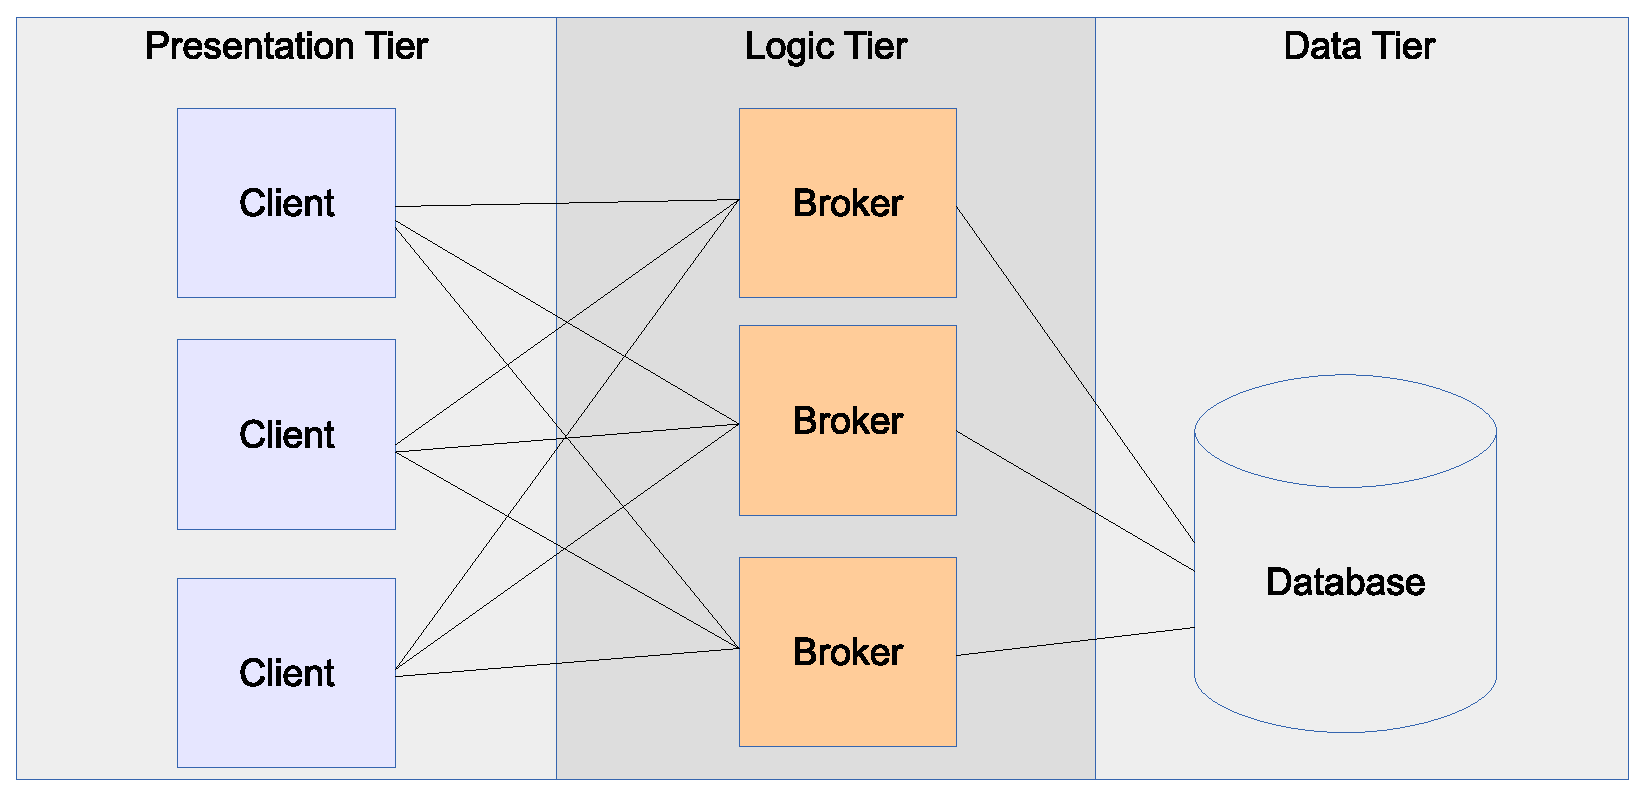
\includegraphics[scale=0.3]{../../drawings/system-overview.eps}
  \end{center}
  \caption{System Overview}
  \label{fig:system-overview}
\end{figure}

\end{frame}

\section{Database}
\begin{frame}
\frametitle{DB Schema}

\end{frame}


\section{Database Schema}
\begin{frame}
\frametitle{Database Schema}
Schema, Stored Procedures
\end{frame}



\section{Messaging System}
\begin{frame}
\frametitle{Server}
\begin{itemize}
\item Threading
\item Java NIO Reactor
\end{itemize}
\end{frame}

\begin{frame}
\frametitle{Client-Middleware Communication}
\begin{itemize}
\item Describe Communication between
\end{itemize}
\end{frame}


\section{Client}
\begin{frame}
Describe the client
\end{frame}


\section{Communication Protocol}
\begin{frame}
\frametitle{Communication Protocol}
Communication Protocol used by client and server
\end{frame}



\section{Management Interface}
\begin{frame}
\frametitle{Management Interface}
Use JMX?
\end{frame}


\section{Measurements}
\begin{frame}
\frametitle{What experiments are performed}


\begin{enumerate}
\item what kind of experiments are performed
\item how to perform measurements
\item where to store measurement results (Format, Use DB, etc)
\end{enumerate}

\end{frame}


\end{document}

